\section{Classic Communication Complexity}
    
    \begin{frame}{Communication Complexity}
        \begin{figure}
            \centering
            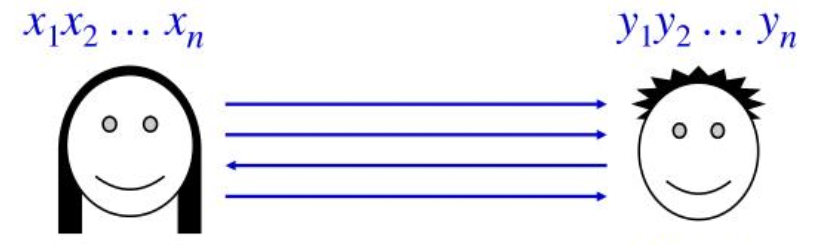
\includegraphics[width=\linewidth]{pics/1.png}
            \caption{Alice and Bob each have an $n$ bit number.}
            \label{fig:my_label}
        \end{figure}
        
        
        \begin{itemize}
        	\uncover<+->{\item They want to compute a function $f(x,y)$}
        	\uncover<+->{\item But with the least amount of communication possible.}

        	
        \end{itemize}
    \end{frame}
    
    \begin{frame}{Equality}
        \begin{example}
        We want to find the least amount of communication necessary to compute the equality function, i.e., 
        \begin{equation*}
            EQ_{n}(x,y) =
    \begin{cases}
        1 & \text{x = y}\\
        0 & \text{o.w.}
    \end{cases}
        \end{equation*}
        \end{example}
    
    
    \uncover<+->{\textbf{Deterministic CC:} $O(n)$.\\
    \quad We can prove - using the fooling set technique -  that communicating the entire input is required to compute the function.}
    \end{frame}
% \begin{frame}{Equality cont.}
%     \uncover<+->{\textbf{2. Non-deterministic CC:} $O(1)$.\\
%     \quad Sending one bit non-deterministically and checking it.\\}\vspace{1cm}
%     \uncover<+->{\textbf{3. Randomized CC:} \\
%     }
%     \uncover<+->{\begin{itemize}
%             \item Private Coin: $O(\log n)$
%         \item Public Coin: $O(1)$

%     \end{itemize}}
% \end{frame}
    \begin{frame}{Disjointness}
        \begin{example}
        Another problem that we discuss is the set disjointness problem. We intrepret the inputs as subsets of $\{1,\dots, n\}$ and we have:
        \begin{equation*}
            DISJ_{n}(x,y) =
    \begin{cases}
        1 & \text{x and y are disjoint}\\
        0 & \text{o.w.}
    \end{cases}
        \end{equation*}
        \end{example}
\uncover<+->{\textbf{Deterministic CC:} $O(n)$.\\
    \quad We can prove - using the rank technique -  that this is the lower bound for the communication needed.}
\end{frame}